\documentclass{beamer}
\usetheme{Warsaw}

\usepackage[utf8]{inputenc}
\usepackage{fancybox}
\usepackage{multimedia} 
\usepackage{subfig}
\usepackage{amsmath}
\usepackage{hyperref}
\hypersetup{
    colorlinks=true,     
    urlcolor=blue
}
\usepackage[all]{xy}
\begin{document}


\title[Stochastik] % (optional, only for long titles)
{Stochastik für Informatiker
\\
\includegraphics[scale=0.5]{img/craps}
}
\subtitle{}
\author[Dr. Johannes Riesterer] % (optional, for multiple authors)
{Dr.  rer. nat. Johannes Riesterer}

\date[KPT 2004] % (optional)
{}

\subject{Stochastik}


\begin{frame}
    \frametitle{Zentraler Grenzwertsatz}
\framesubtitle{}

\begin{block}{Motivation}
Welche Verteilung hat das arithmetische Mittel $S_n:= \frac{1}{n} \sum_{i=1}^n X_i$?
\end{block}
\begin{block}{Motivation}
Wie und gegen was konvergiert $P_{S_n}$? 
\end{block}

 \end{frame}




\begin{frame}
    \frametitle{Zentraler Grenzwertsatz}
\framesubtitle{}

\begin{block}{Konvergenz von W-Maßen}
Was bedeutet Konvergenz einer Folge von Wahrscheinlichkeitsmaßen?
\end{block}
\begin{block}{Inspiration: Gleichmässige Konvergenz von Funktionen}
Eine Folge von Funktionen $f_n: A \subset \mathbb{R}^n \to \mathbb{R}$ konvergiert gleichmässig gegen eine Funktion $f$, falls 
\begin{align*}
\lim_{n \to \infty} ||f_n(x) -f(x) || = 0
\end{align*}
für alle $x \in A$.
\end{block}

 \end{frame}

\begin{frame}
    \frametitle{Allgemeine Wahrscheinlichketisräume/Nachtrag}
\framesubtitle{}

\begin{block}{Konvergenz von W-Maßen}
Sei $(\Omega, \mathcal{A})$ ein Wahrscheinlichkeitsraum und $P_n : \Omega \to [0,1]$ eine folge von Wahrscheinlichkeits-Maßen. Die Folge konvergiert gegen
das Wahrscheinlichkeits-Maß $P: \Omega \to [0,1]$, falls 
\begin{align*}
\lim_{n \to \infty} \int_\Omega f dP_n = \int_\Omega f dP
\end{align*}
für alle messbaren Funktionen $f: \Omega \to \mathbb{R}$.
\end{block}
 \end{frame}



\begin{frame}
    \frametitle{Zentraler Grenzwertsatz}
\framesubtitle{}

\begin{block}{Zentraler Grenzwertsatz}
Sei $(\Omega, \mathcal{A}, P)$ ein Wahrscheinlichkeitsraum und $X_n :  \Omega \to \mathbb{R}$  eine folge stochastisch unabhängiger, identisch verteilter, reeller Zufallsvariablen mit $E(X_n) = \mu$ und $V(X_n)= \sigma^2$. Dann gilt für das arithmetische Mittel $S_n:= \frac{1}{n} \sum_{i=1}^n X_i$
\begin{align*}
P_{ \frac{\sqrt{n}}{\sigma} (S_n-\mu)} \to P_{N(0,1)}
\end{align*}
wobei $ P_{N(0,1)}$ das Wahrscheinlichkeits-Maß mit der Dichte $ \frac {1}{ \sqrt{2\pi}}e^{- \frac {1}{2} x^2}$ ist.
\end{block}

 \end{frame}



\begin{frame}
    \frametitle{Zentraler Grenzwertsatz}
\framesubtitle{}

\begin{block}{Erzeugende Funktion}
Sei $(\Omega, \mathcal{A}, P)$ ein Wahrscheinlichkeitsraum und $X :  \Omega \to \mathbb{R}$  eine reelle Zufallsvariable. Dann heißt die Funktion 
\begin{align*}
\psi_X(t) := \mathbb{E}(e^{tX}), \; t \in I \subset \mathbb{R}
\end{align*}
erzeugende Funktion zu $X$ bzw. $P_X$.
\end{block}

\begin{block}{Stetigkeitssatz von  Lévy }
Sei $(\Omega, \mathcal{A}, P)$ ein Wahrscheinlichkeitsraum so wie  $X$ und $X_n :  \Omega \to \mathbb{R}$   reelle Zufallsvariablen mit erzeugenden Funktionen $\psi$ und $\psi_{n}$. Dann gilt:
\begin{align*}
\psi_n \to \psi \Rightarrow P_{X_n} \to P_X 
\end{align*}
\end{block}

 \end{frame}

\begin{frame}
    \frametitle{Zentraler Grenzwertsatz}
\framesubtitle{}
\begin{block}{Eigenschaften erzeugender Funktionen}
\begin{itemize}
\item $\psi_X(t) = \sum_{k= 0}^n \frac{\mathbb{E}(X^k)}{k!} t^k$ für $|t| \leq \delta$ (Taylor).
\item $e^{\frac{t^2}{2}}$ ist die erzeugende Funktion von $ P_{N(0,1)}$.
\item $\psi_{X +Y} = \psi_X \cdot \psi_Y$
\end{itemize}

\end{block}


 \end{frame}




\begin{frame}
    \frametitle{Zentraler Grenzwertsatz}
\framesubtitle{}

\begin{block}{Beweis Zentraler Grenzwertsatz}
\begin{itemize}
\item $|t| \leq \delta$
\item $\psi(t)$ erzeugende Funktion von $X_n$.
\item $Y_n := \frac{X_n - \mu}{\sigma}$. Dann ist $\mathbb{E}(Y_n) = 0$ und $\mathbb{V}(Y_n) = 1$.
\item $\psi^*(t)$ erzeugende Funktion von $Y_n$.
\item $\psi_n(t)$ erzeugende Funktion von $\frac{Y_n}{\sqrt{n}}$. Dann ist $\psi_n(t) = \psi^*(\frac{t}{\sqrt{n}})$ 
\end{itemize}
\begin{align*}
\psi_n(t) &= \psi^*(\frac{t}{\sqrt{n}}) =  \sum_{k= 0}^n \frac{t^k }{k! \sqrt{n}^k} \mathbb{E}(Y_i^k) \\
& = 1 + \frac{t^2}{2n} +  \underbrace{\sum_{k= 3}^n \frac{t^k }{k! \sqrt{n}^k} \mathbb{E}(Y_i^k)}_{=:R_n} 
\end{align*}
\end{block}

 \end{frame}



\begin{frame}
    \frametitle{Zentraler Grenzwertsatz}
\framesubtitle{}

\begin{block}{Beweis Zentraler Grenzwertsatz}
\begin{align*}
R_n \leq \frac{1}{n \sqrt{n}} (\psi^*(\delta)  + \psi^*(-\delta) ) \rightarrow 0  \text{ für } n \to \infty
\end{align*}
Für $T_n := \frac{\sqrt{n}}{\sigma}(S_n - \mu)$ erhält man damit
\begin{align*}
\psi_{T_n}(t) = (\psi_n)(t))^n = \biggl(  1 + \frac{t^2}{2n} + R_n(t) \biggr)^n \rightarrow e^{\frac{t^2}{2}} \text{ für } n \to \infty
\end{align*}
Mit dem Stetigkeitssatz von Levy folgt der zentrale Grentzwertsatz.
\end{block}

 \end{frame}



\begin{frame}
    \frametitle{Zentraler Grenzwertsatz}
\framesubtitle{}

\begin{block}{Fourier-Reihe}
Für eine $2\pi$ periodische Funktion $f: \mathbb{R} \to \mathbb{C}$  heißt 
\begin{align*}
Sf_n(x) := \sum_{k= -n}^{n} \hat{f}(k) \cdot e^{ikx} 
\end{align*}
die Fourier-Reihe von $f$ vom Grad $n$ mit den den Fourier-Koeffizienten
\begin{align*}
\hat{f}(k) := \frac{1}{2 \pi} \int_{[0, 2 \pi]} f(t) \cdot e^{-ikt} \; dt
\end{align*}
\end{block}

 \end{frame}


\begin{frame}
    \frametitle{Zentraler Grenzwertsatz}
\framesubtitle{}

\begin{block}{Fourier-Reihe}
Ist $f$  $2\pi$-periodisch,  stetig und stückweise stetig differenzierbar, so konvergiert die Fourierreihe gleichmässig gegen $f$, es gilt dann also 
\begin{align*}
\lim_{n \to \infty} \max_x |Sf_n(x) -f(x) | = 0
\end{align*}
\end{block}

 \end{frame}



\begin{frame}
    \frametitle{Zentraler Grenzwertsatz}
\framesubtitle{}

\begin{block}{Fourier-Reihe - Interpretation}
Es ist $e^{-ikt} := \cos (k t) + i \sin(kt)$ und 
\begin{align*}
  \frac{1}{2 \pi}  \int_{[0, 2 \pi]}  e^{-ilt} \cdot e^{-ikt} \; dt = \begin{cases} 1 \text{ für k = l}  \\ 0 \text{ sonst }\end{cases}
\end{align*}
Die Funktionen  $e^{-ikt}$ bilden bezüglich des Skalarproduktes $\langle f, g \rangle : =\frac{1}{2 \pi}  \int_{[0, 2 \pi]}  f(t) \cdot g(t) \; dt$ eine orthonormalbasis der $2\pi$-periodisch, stetig und stückweise stetig differenzierbaren Funktionen.
\end{block}
 \end{frame}


\begin{frame}
    \frametitle{Zentraler Grenzwertsatz}
\framesubtitle{}

\begin{block}{Fourier-Reihe einer rellen Funktion}
Ist $f :\mathbb{R} \to \mathbb{R}$ eine reelle Funktion, so gilt
\begin{align*}
Sf_n(x) := \frac{a_0}{2} + \sum_{k= 1}^{n} a_k \cos (kx) + b_k \sin (kx)  
\end{align*}
mit den Koeffizienten
\begin{align*}
a_k := \frac{1}{ \pi} \int_{-\pi}^{\pi} f(x) \cos (kx)\; dx \\
b_k := \frac{1}{ \pi} \int_{-\pi}^{\pi} f(x) \sin (kx)\; dx
\end{align*}

\end{block}
\begin{block}{Beweisidee}
Ersetze   $e^{-ikt} = \cos(kt) + i \sin (kt)$ und setze $a_k := \hat{f}(k) + \hat{f}(-k)$ und $b_k :=  i(\hat{f}(k) - \hat{f}(-k))$.
\end{block}
 \end{frame}


\begin{frame}
    \frametitle{Zentraler Grenzwertsatz}
\framesubtitle{}

\begin{block}{Beispiel}
\begin{align*}
f(t) = \begin{cases} h, & \mbox{ wenn } 0\leq  t <T/2 \\ -h, & \mbox{ wenn } T/2 \leq t < T \end{cases}  \qquad f(t + T) = f(t)
\end{align*}
\end{block}
\begin{figure}[htp]
      \centering
    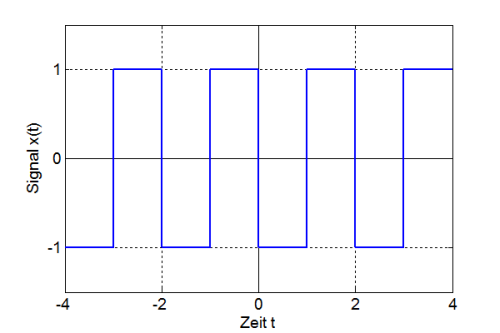
\includegraphics[width=0.45\textwidth]{img/rechteck}
      \caption{Quelle: Wikipedia}
\end{figure}

 \end{frame}

\begin{frame}
    \frametitle{Zentraler Grenzwertsatz}
\framesubtitle{}

\begin{block}{Beispiel}
\begin{align*}
Sf(t)=& \tfrac{4h}{\pi}\left[\sin \omega t+\tfrac{1}{3}\sin3 \omega t+\tfrac {1}{5}\sin5 \omega t+\tfrac{1}{7}\sin7 \omega t+ \cdots\right]\\
=& \tfrac{4h}{\pi} \sum_{k=1}^\infty \dfrac{ \sin\left( (2k-1)\omega t \right) }{2k-1} \\
& \omega = 2 \pi \cdot f
\end{align*}
\end{block}
\begin{figure}[htp]
      \centering
    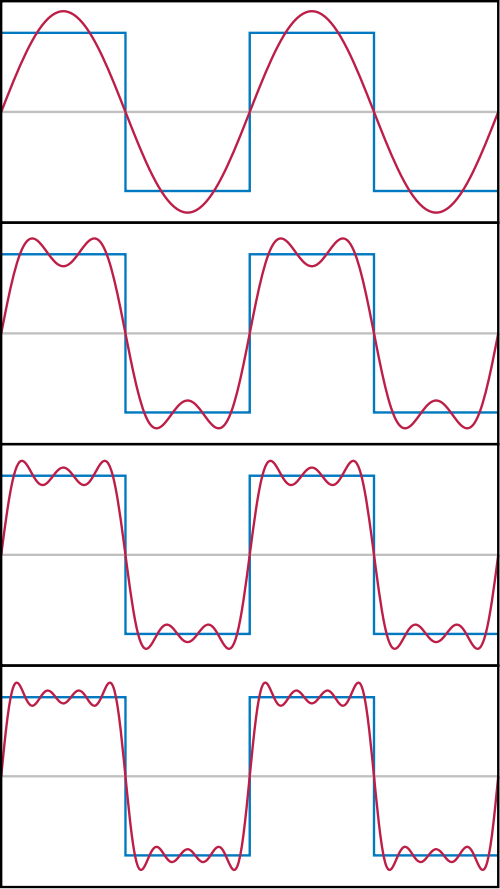
\includegraphics[width=0.15\textwidth]{img/fourier_example}
      \caption{Quelle: Wikipedia}
\end{figure}

 \end{frame}



\begin{frame}
    \frametitle{Zentraler Grenzwertsatz}
\framesubtitle{}

\begin{figure}[htp]
      \centering
    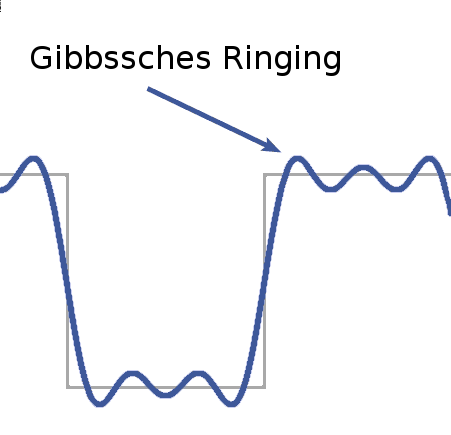
\includegraphics[width=0.35\textwidth]{img/Gibb}
      \caption{Quelle: Wikipedia}
\end{figure}

 \end{frame}



\begin{frame}
    \frametitle{Zentraler Grenzwertsatz}
\framesubtitle{}

\begin{block}{Fouriertransformation}
Sei $f: \mathbb{R}^n \to \mathbb{R}$ eine integrierbare Funktion. Die (kontinuierliche) Fourier-Transformierte ist definiert durch
\begin{align*}
\hat{ f}(y) = \frac{1}{\left(2\pi \right)^{n/2}} \int_{\mathbb{R}^n} f(x)\,e^{-i  <y, x>} \, d x,
\end{align*}
(Verallgemeinerung der Fourierkoeffizienten für nicht ganzzahlige Frequenzanteile).
\end{block}

 \end{frame}


\begin{frame}
    \frametitle{Zentraler Grenzwertsatz}
\framesubtitle{}

\begin{block}{Umkehrsatz}
Ist $f: \mathbb{R}^n  \to  \mathbb{R}$ und $\hat{ f}$ integrierbar, gilt
\begin{align*}
f(x) = \frac{1}{\left(2\pi \right)^{n/2}} \int_{\mathbb{R}^n}\hat{ f}(y) \,e^{i  <x, y>} \, d y,
\end{align*}
fast überall.
\end{block}
 \end{frame}



\begin{frame}
    \frametitle{Zentraler Grenzwertsatz}
\framesubtitle{}

\begin{block}{Stetigkeitssatz von Levy}
Mit $\varphi_{X} := \mathbb{E}(e^{i tx})$  ist $\varphi _{X}(-it)=\psi_{X}(t)$ und der Stetigkeitssatz von Levy folgt aus dem Umkehrsatz.
\end{block}
 \end{frame}





\frame{\titlepage}
\begin{frame}
    \frametitle{Zentraler Grenzwertsatz}
\framesubtitle{}


\begin{block}{Motivation}

\end{block}

 \end{frame}


\end{document}
